% !TeX root = ../dd.tex
\section{Overview}
Here we represent an high level overview of the S\&C architecture: 

\begin{figure}[H]
    \centering
    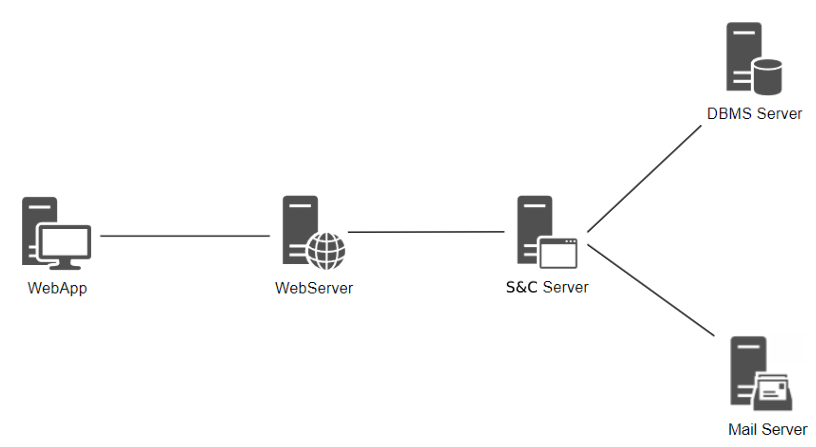
\includegraphics[width=\textwidth]{../images/Overview.PNG}
    \caption{S\&C overview}
    \label{fig:S\&C overview}
\end{figure}

Client side:
\begin{itemize}
\item \textbf{WebApp:} allows all users to access the S\&C platform. It enables user to perform various operations such as registration, login in, creating an internship or a CV etc.
\end{itemize}
Server side: 
\begin{itemize}
\item \textbf{Web Server:} handles the communication with users by receiving and processing their commands, which are then directed to the S\&C server. 
\item \textbf{S\&C server:} manages most of the platform functionalities by using different components which are created to do a specific job. It facilitates the communication between the Web Server and Databases/APIs. It is also replicated across multiple machines to handle a high volume of requests.
\item \textbf{DBMS Server:} contains data of students, universities, companies, CVs and various information obtained through questionnaires compiled by students. 
\item \textbf{Mail Server:} is responsible for sending confirmation eMails and all the notification regarding the reccomendation process.
\end{itemize}

\section{Component view}
\begin{figure}[H]
    \centering
    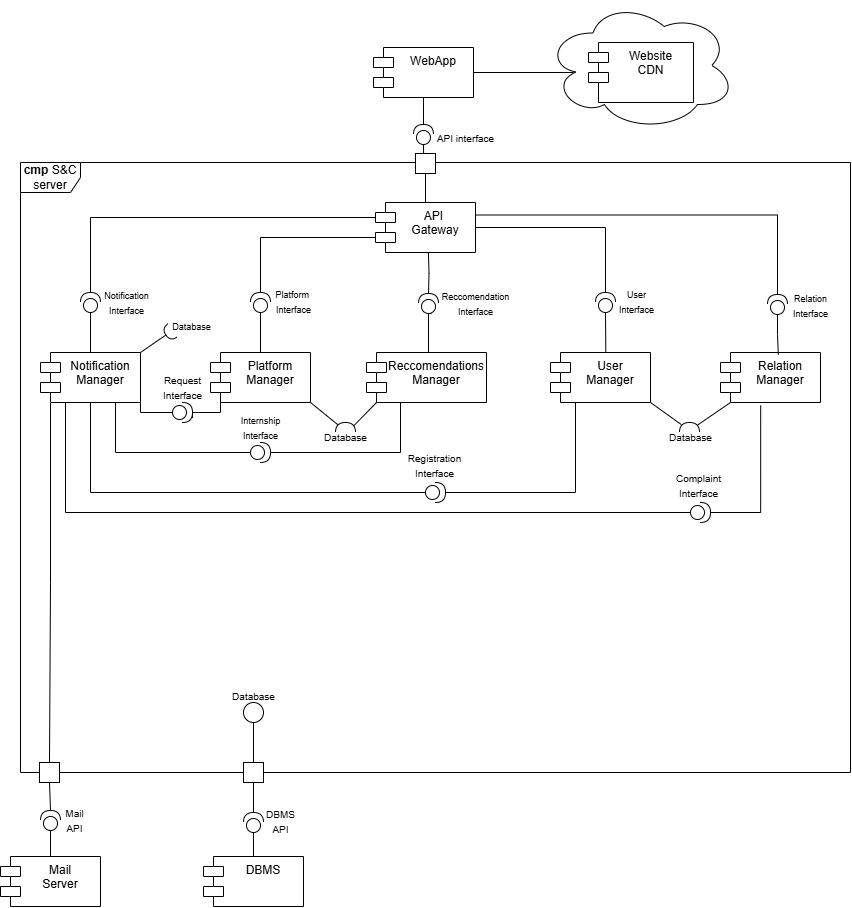
\includegraphics[width=\textwidth]{../images/Component_Diagram2.drawio.png}
    \caption{Component View Diagram}
    \label{fig:Component View Diagram}
\end{figure}
In the figure above it's shown the component view diagram of the platform, where it is represented how the external components of S\&C communicate with the S\&C server. Looking at the high level part of the diagram the components are:
\begin{itemize}

    \item{\textbf{WebApp:}} which is an external access point for users, allowing the communication with the S\&C server through an API interface.
    \item{\textbf{Website CDN:}} which is responsible for improving the distribution of web content to end users.
    \item{\textbf{API interface:}} which is responsible for connecting the presentation layer (WebApp) with the application layer (S\&C server), which is coordinated by an API Gateway.
    \item{\textbf{Mail Server:}} is responsible for sending notification to the users such as registration confirmation eMails, new student Cv notification to companies or new internship posted notifications to students.
    \item{\textbf{DBMS:}} which is the data warehouse of the system containing data from the questionnaires, user's CV, company's data and internship related data.
\end{itemize}
Looking the diagram at a lower level, it shows all the components inside the server:
\begin{itemize}
    \item \textbf{API Gateway:} is a must have component which manages all the communication between the user and the platform. Users interact with S\&C through the API interface, and the API Gateway directs the requests to the appropriate component. 
    \item \textbf{Notification Manager:} handles all the notifications that are to be sent to users. In particular it sends a message to: companies every time a student who is fit to their needs has registered, to students every time a company posts an interesting internship or to universities every time one of the two parties complains. To know which user to send the message to, the notification manager needs to interact with the DBMS API. 
    \item\textbf{Platform Manager:} it manages all the aspects related to users necessities. For example, it allows students to provide their own information to create their personalized CV, allows student to join internships or allows all the parties to chat and communicate.
    \item \textbf{Reccomendations Manager:} is a component that handles the reccomendation process where through the use of statistical analysis and word searching mechanism recommends to student the most fit internships available, or recommends to companies new students that added their CV information.
    \item\textbf{User Manager:} this component handles the registration and log in of users. Whenever a new user wants to create an account a request is forwarded to this component by the API Gateway. Then the User Manager handles the request by sending through the registration interface and the notification manager a confirmation email. Once the email has been confirmed the component through the model interface adds the new user's information to the DBMS, including his topic preferences. For the login process the API Gateway forwards the request to the User manager, which communicates with the  DBMS to retrieve the user's data.
    \item \textbf{Relation Manager:} this component manages the interactions between users letting them complain about problems or informing other parties about the current status of the internship.
\end{itemize}

\section{Deployment view}

\begin{figure}[H]
    \centering
    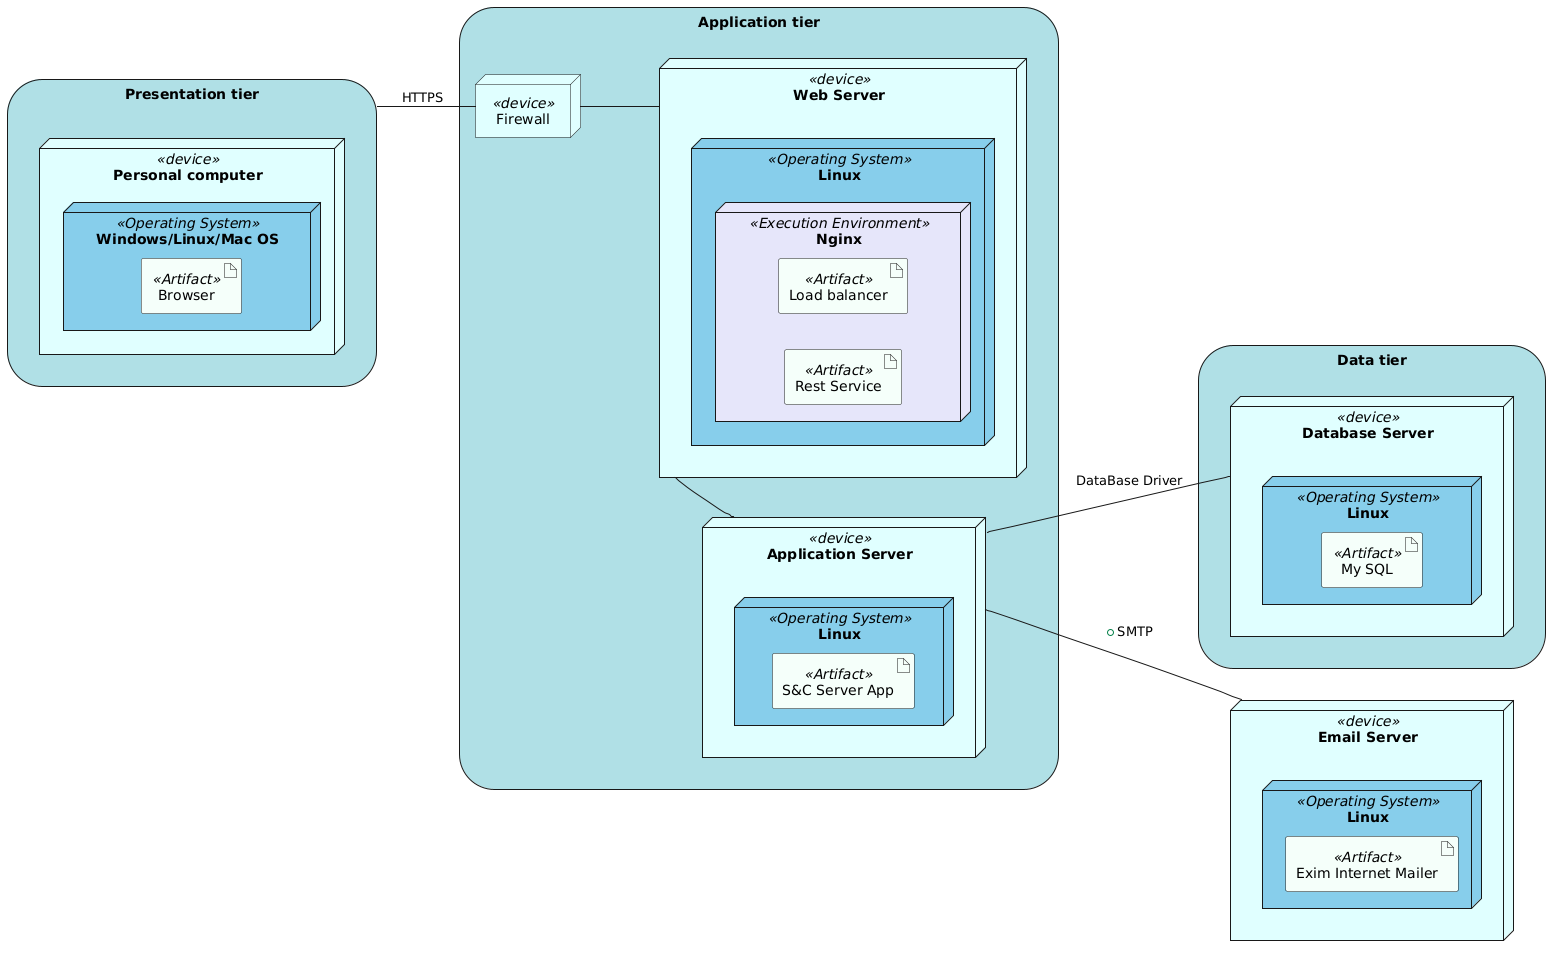
\includegraphics[width=\textwidth]{../images/Deployment_diagram.png}
    \caption{Deployment Diagram}
    \label{fig:Deployment Diagram}
\end{figure}

\begin{description}[noitemsep,    % Niente spazio aggiuntivo tra le righe
                    itemsep=1em, % Spaziatura verticale tra un “item” e il successivo
                    labelsep=0.5em] % Distanza tra il "titolino" e il testo
                    \item[\textbf{Personal computer:}] Students and companies can access the platform using any browser installed on any computer. Access is also granted via any device that allows access to a web browser, such as a smartphone, tablet or smart TV. The browser will communicate with the Web Server
  \item[\textbf{Web Server:}] The Web Server serves as the entry point for users accessing the Application Server’s services via a web browser. It does not process business logic itself; rather, it balances incoming requests among various Application Servers to efficiently handle high volumes of user traffic. Additionally, it provides the client’s browser with the necessary HTML, JSON, JavaScript, and CSS files to render the pages.
  \item[\textbf{Firewall:}] Security system that monitors and filters incoming and outgoing network traffic based on predefined rules. It acts as a barrier between a trusted internal network and untrusted external networks, helping to block malicious traffic and unauthorized access.
  \item[\textbf{Application Server:}] The Application Server hosts the system’s entire business logic. It communicates with clients over HTTPS, facilitated by the Web Server. The Dashboard Manager directs incoming requests from the Web Server to the appropriate module, and the model gateway manages communication with the Database Server. This server node is replicated to accommodate high user traffic.
  \item[\textbf{Database Server:}] All data concerning users, companies and universities are stored in the Database Server and managed by MySQL.
The various Application Servers can retrieve information on this node via the model module and the database driver.
  \item[\textbf{Email Server:}] The Email Server handles all notifications that are sent by e-mail. When there is a notification, such as that of a compatible internship offer, the Application Server contacts the Email Server through SMTP protol to send the email to the recipient user
\end{description}


\pagebreak

\section{Runtime view}
The following sequence diagrams represent the dynamics of interaction between components.\\
Sequence diagrams from \ref{{RW1}} to \ref{{RW9}} are the realizations of the corresponding use cases in the RASD document.\\


\begin{enumerate}[label=\textbf{RW\arabic*}:,ref=RW\arabic*,leftmargin=1.3cm]

  \labelleditem{
      \textbf{}
      \begin{figure}[H]
        \centering
        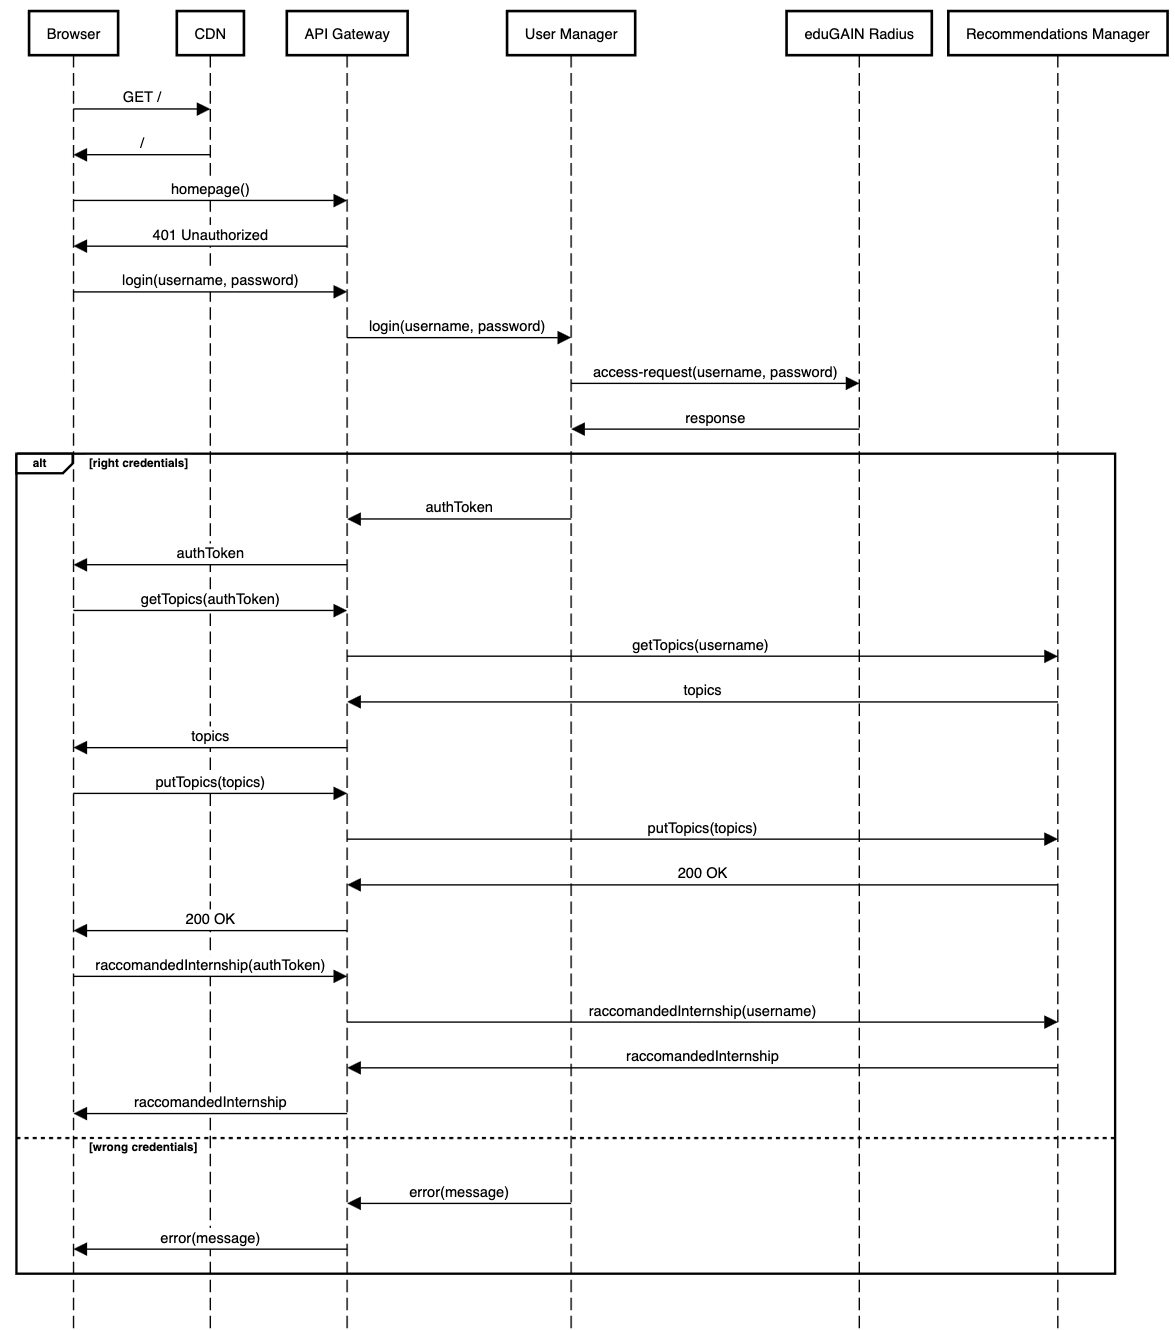
\includegraphics[width=0.8\textwidth]{dd/assets/runtime-sequence-diagrams/1-student-first-login.png}
        \caption{Student’s first platform access.}
        \label{fig:Student’s first platform access}
    \end{figure}
    \pagebreak
  }
  
  \labelleditem{
      \textbf{}
      \begin{figure}[H]
        \centering
        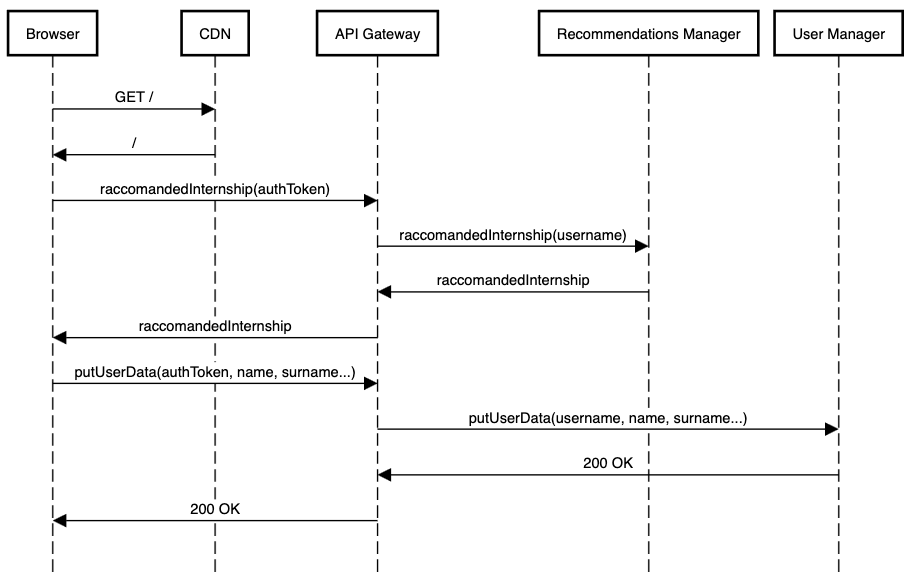
\includegraphics[width=0.8\textwidth]{dd/assets/runtime-sequence-diagrams/2-student-initial-form.png}
        \caption{Student inserts his CV information in the InitialForm.}
        \label{fig:Student inserts his CV information in the InitialForm}
    \end{figure}
    \pagebreak
  }

    \labelleditem{
        \textbf{}
        \begin{figure}[H]
            \centering
            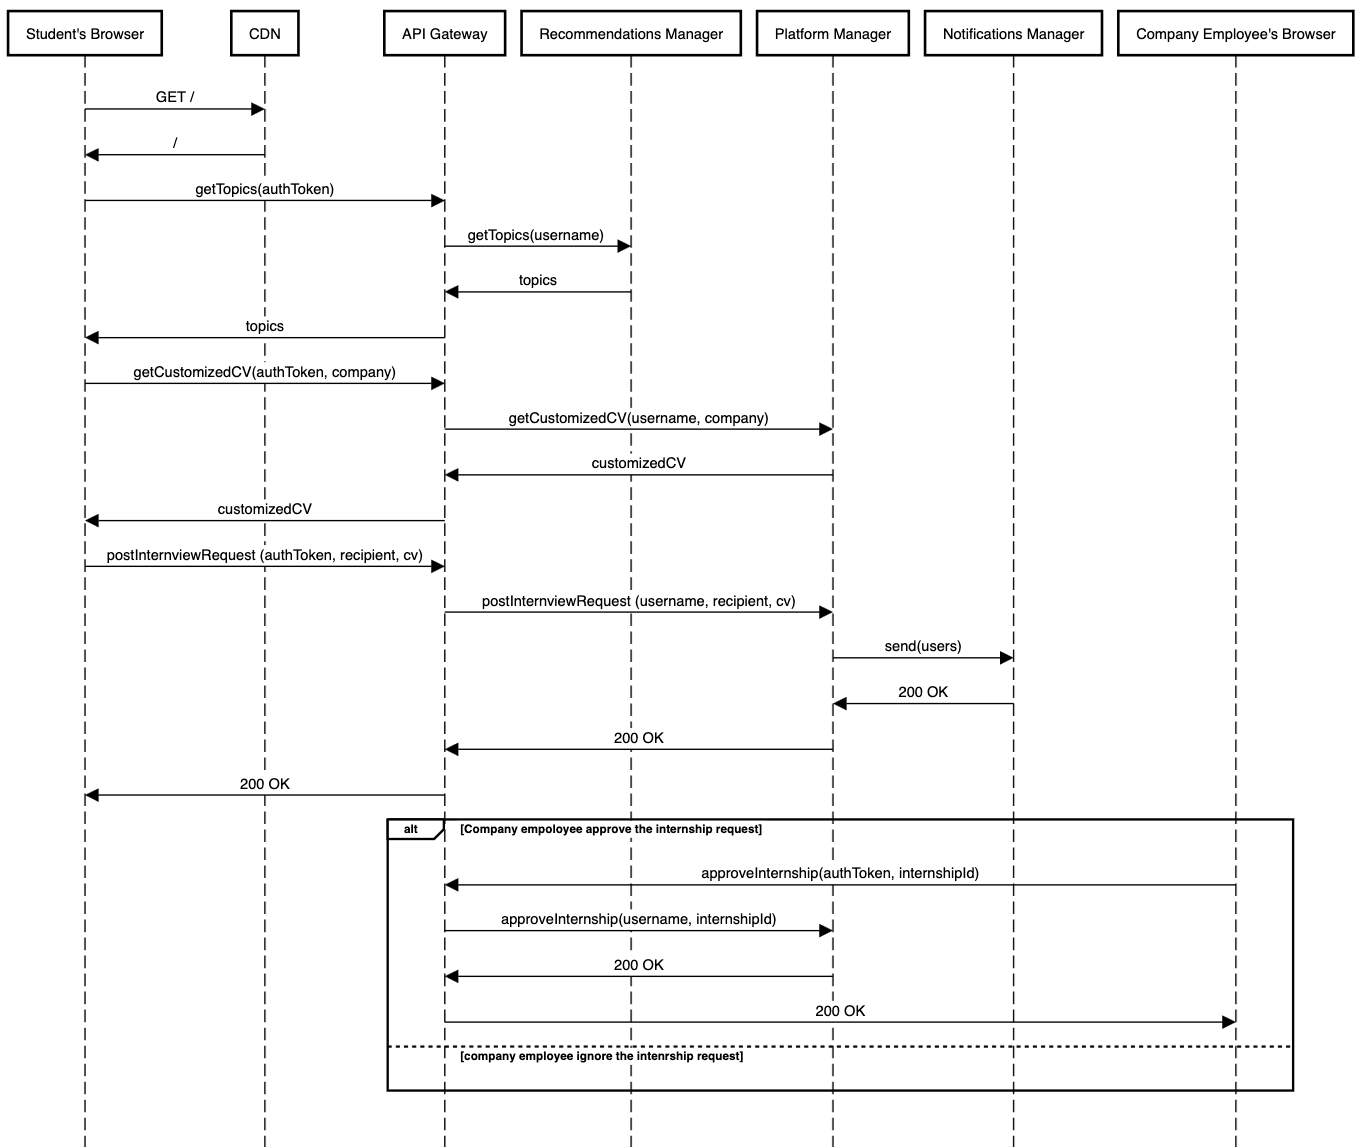
\includegraphics[width=0.8\textwidth]{dd/assets/runtime-sequence-diagrams/3-students-ask-for-internship.png}
            \caption{Student search through the internships and contact the company.}
            \label{fig:Student search through the internships and contact the company}  
        \end{figure}
        \pagebreak
  }
  
  \labelleditem{
      \textbf{}
      \begin{figure}[H]
        \centering
        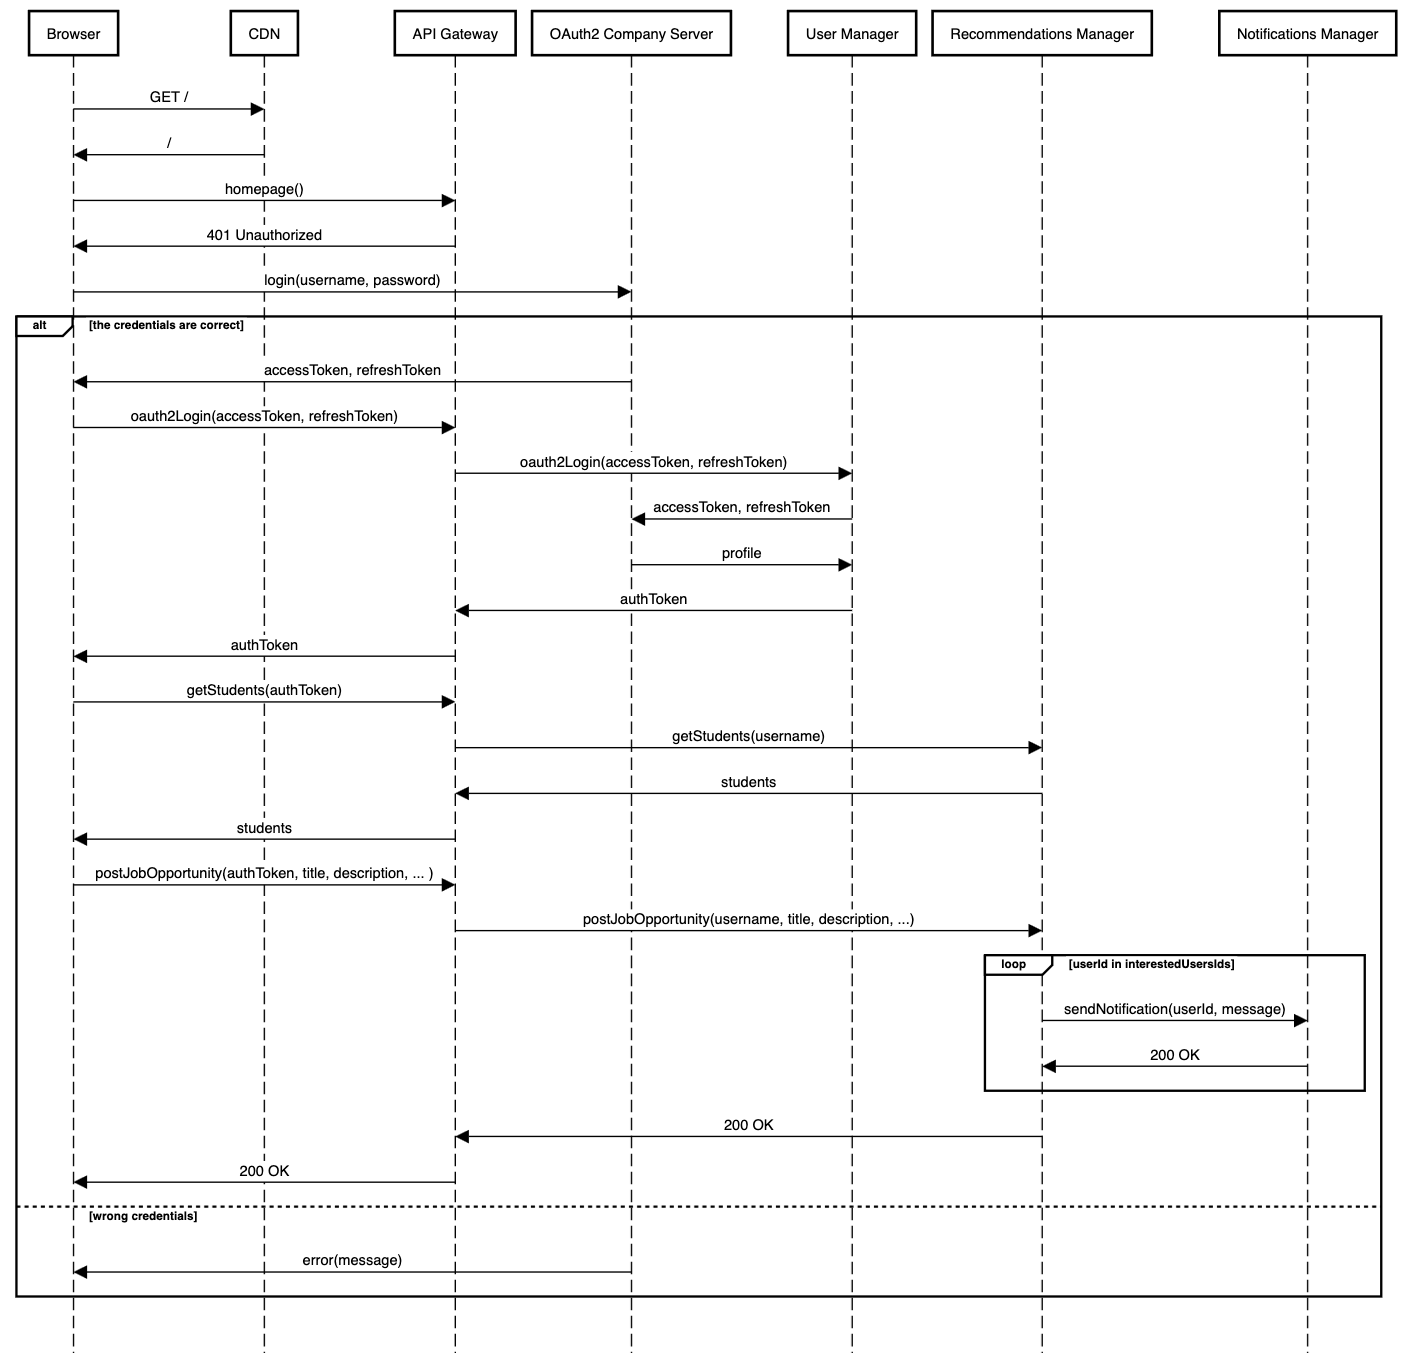
\includegraphics[width=0.8\textwidth]{dd/assets/runtime-sequence-diagrams/4-employee-new-internship.png}
        \caption{A company publishes an advertisement about the internships they are offering.}
        \label{fig:A company publishes an advertisement about the internships they are offering}
    \end{figure}
    \pagebreak
  }

  \labelleditem{
      \textbf{}
      \begin{figure}[H]
        \centering
        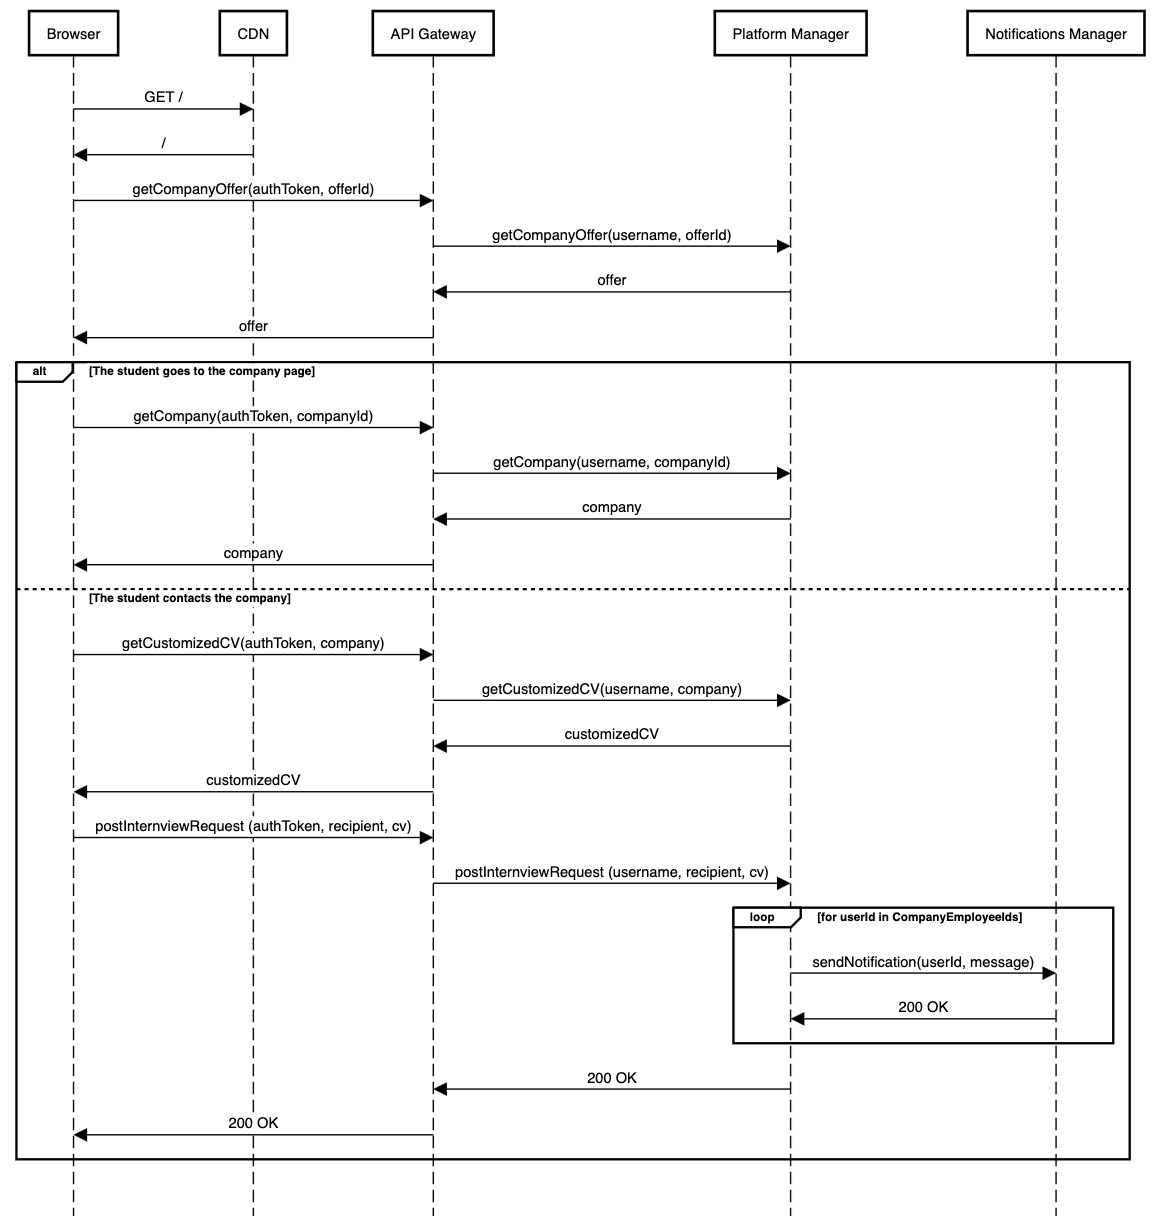
\includegraphics[width=0.8\textwidth]{dd/assets/runtime-sequence-diagrams/5-student-receive-notification.png}
        \caption{A student receive a notification about the availability of an internship that might interest her.}
        \label{fig:A student receive a notification about the availability of an internship that might interest her}
    \end{figure}
    \pagebreak
  }
  \labelleditem{
      \textbf{}
      \begin{figure}[H]
        \centering
        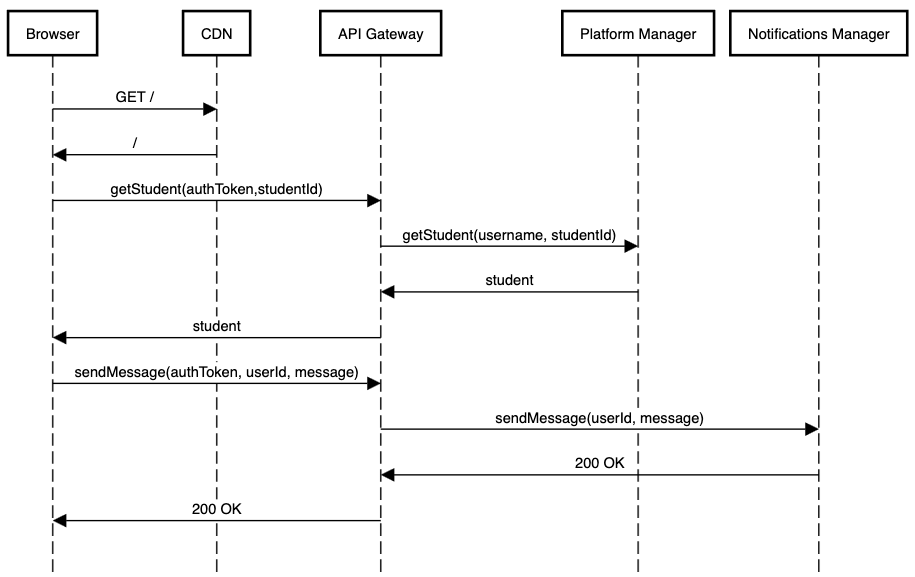
\includegraphics[width=0.8\textwidth]{dd/assets/runtime-sequence-diagrams/6-company-receive-a-notification.png}
        \caption{A company receives a notification about the availability of a student CV corresponding to their needs.}
        \label{fig:A company receives a notification about the availability of a student CV corresponding to their needs}
    \end{figure}
    \pagebreak
  }
  \labelleditem{
      \textbf{}
      \begin{figure}[H]
        \centering
        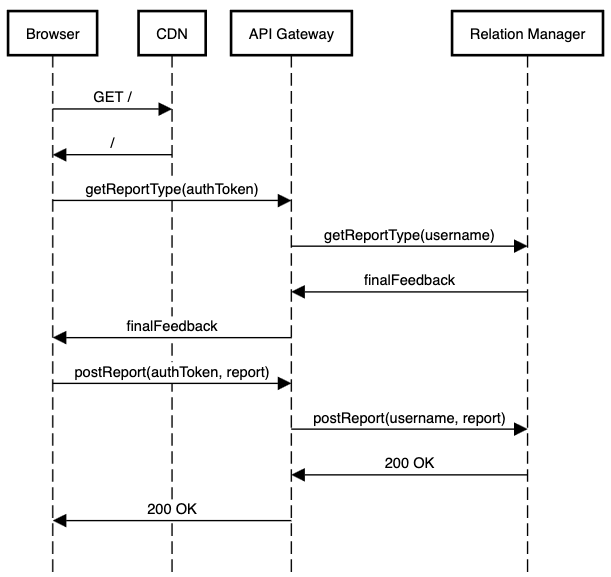
\includegraphics[width=0.8\textwidth]{dd/assets/runtime-sequence-diagrams/7-student-feedback.png}
        \caption{Student gives final feedback about the internship.}
        \label{fig:Student gives final feedback about the internship}
    \end{figure}
    \pagebreak
  }
  \labelleditem{
      \textbf{}
      \begin{figure}[H]
        \centering
        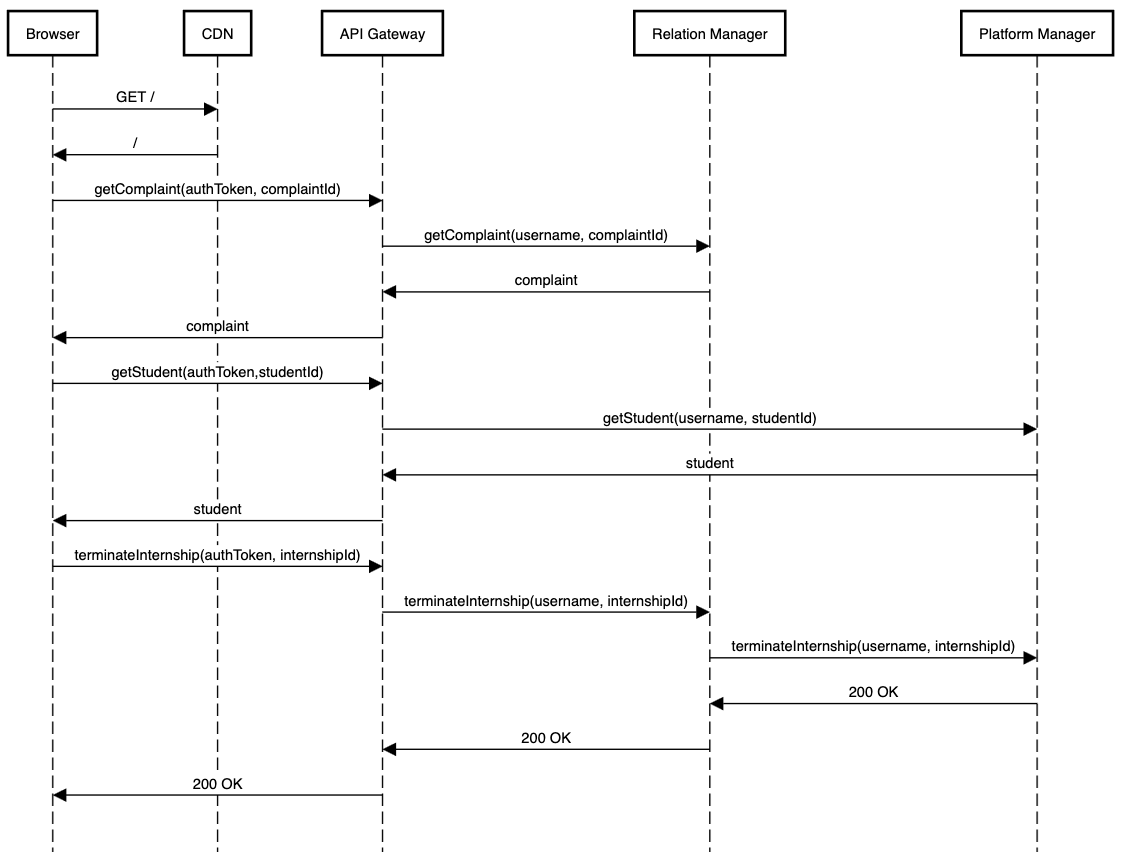
\includegraphics[width=0.8\textwidth]{dd/assets/runtime-sequence-diagrams/8-terminate-internship.png}
        \caption{The University receives the request to end an internship from a student and contacts the company to end it.}
        \label{fig:The University receives the request to end an internship from a student and contacts the company to end it}
    \end{figure}
    \pagebreak
  }
  \labelleditem{
      \textbf{}
      \begin{figure}[H]
        \centering
        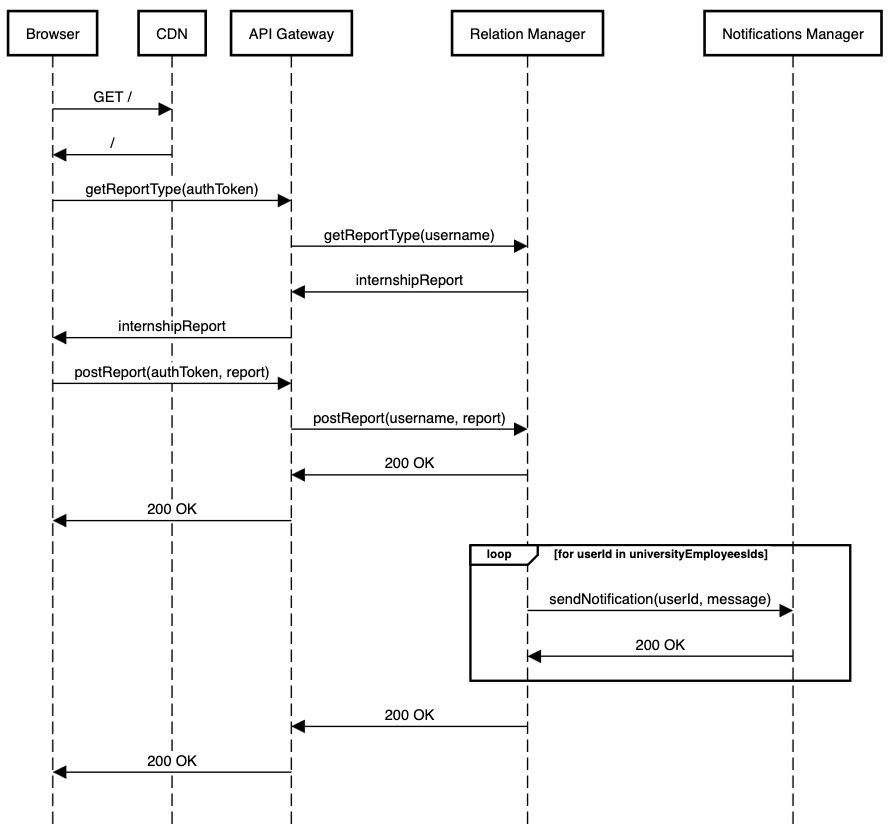
\includegraphics[width=0.8\textwidth]{dd/assets/runtime-sequence-diagrams/9-student-opens-a-complaint.png}
        \caption{Student complains with the university on the "Report Area" about his ongoing internship.}
        \label{fig:Student complains with the university on the "Report Area" about his ongoing internship}
    \end{figure}
    \pagebreak
  }
  \labelleditem{
      \textbf{}
      \begin{figure}[H]
        \centering
        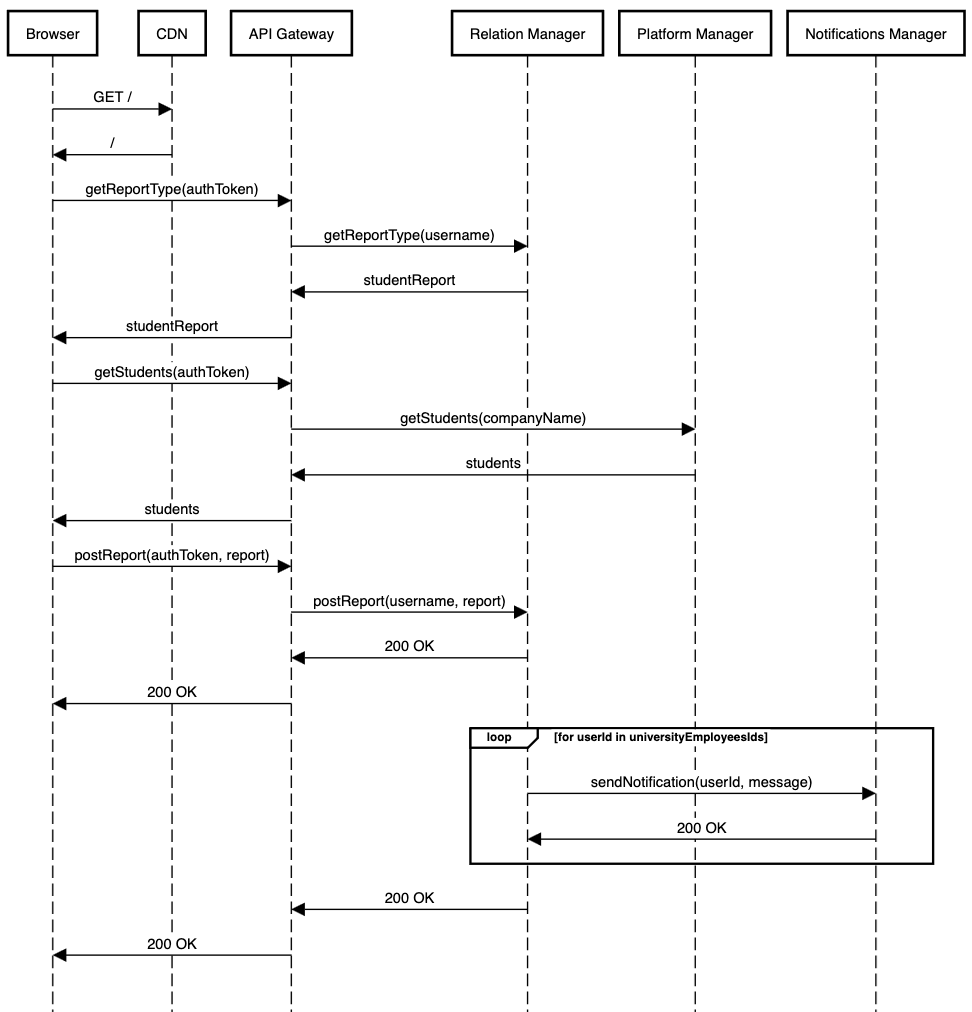
\includegraphics[width=0.8\textwidth]{dd/assets/runtime-sequence-diagrams/10-company-employee-opens-a-complaint.png}
        \caption{The company complains about the student taking the internship.}
        \label{fig:The company complains about the student taking the internship}
    \end{figure}
    \pagebreak
  }

  
\end{enumerate}

\section{Component interfaces}
Here the most relevant interfaces exposed by components are described, including all the operations
seen in the previous diagrams:
\begin{itemize}
    \item \textbf{API Gateway}
          \begin{itemize}
              \item \textbf{login(username: String, password: String): String?}
              \item \textbf{getTopics(authToken: String): List<Topic>}
              \item \textbf{putTopics(authToken: String): Void}
              \item \textbf{raccomandedInternship(authToken: String): List<Internship>}
              \item \textbf{putUserData(authToken: String, name: String, surname: String, ...): Void}
              \item \textbf{oauth2Login(accessToken: String, refreshToken: String): Void}
              \item \textbf{getStudents(authToken: String): List<Student>}
              \item \textbf{postJobOpportunity(authToken: String, title: String, description: String, ... ): Void}
              \item \textbf{getCustomizedCV(authToken: String, company: String): CV}
              \item \textbf{postInterviewRequest (authToken: String, recipient: String, cv: CV): Void}
              \item \textbf{approveInternship(authToken: String, internshipId: ID): Void}
              \item \textbf{getCompanyOffer(authToken: String, offerId: ID): Offer?}
              \item \textbf{getCompany(authToken: String, companyId: ID): Company?}
              \item 
              \textbf{getStudent(authToken: String, studentId: String): Student?}
              \item 
              \textbf{sendMessage(authToken: String, userId: ID, message: String): Void}
              \item \textbf{getReportType(authToken: String): ReportType}
              \item \textbf{postReport(authToken: String, report: Report): Void}
              \item \textbf{getComplaint(authToken:String, complaintId: ID): Complaint?}
              \item \textbf{terminateInternship(authToken: String, internshipId: ID): Void}
          \end{itemize}
             
    \item \textbf{User Manager Interface}
          \begin{itemize}
              \item \textbf{login(username: String, password: String): String?}
              \item \textbf{oauth2Login(accessToken: String, refreshToken: String)}
              \item \textbf{putUserData(username: String, name: String, surname: String, ...): Void}
          \end{itemize}
          
    \item \textbf{Recommendations Manager Interface}
        \begin{itemize}
            \item \textbf{getTopics(username: String): List<Topic>}
            \item \textbf{putTopics(username: String): Void}
            \item \textbf{raccomandedInternship(username: String): List<Internship>}
            \item \textbf{getStudents(username: String): List<Students>}
            \item \textbf{postJobOpportunity(username: String, title: String, description: String, ... ): Void}
        \end{itemize}

              
    \item \textbf{Notifications Manager Interface}
        \begin{itemize}
            \item \textbf{sendMessage(userId: ID, message: String): Void}
            \item \textbf{sendNotification(userId: ID, message: String): Void}
        \end{itemize}
          
    \item \textbf{Platform Manager Interface}
        \begin{itemize}
            \item \textbf{getCustomizedCV(username: String, company: String): CV}
            \item \textbf{postInterviewRequest (username: String, recipient: String, cv: CV): Void}
             \item \textbf{approveInternship(username: String, internshipId: ID): Void}
             \item \textbf{getCompanyOffer(username: String, offerId: ID): Offer?}
             \item \textbf{getCompany(username: String, companyId: ID): Company?}
             \textbf{getStudent(username: String, studentId: String):   Student?}
             \item \textbf{terminateInternship(username: String, internshipId: ID): Void}
        \end{itemize}

    \item \textbf{Relation Manager Interface}
    \begin{itemize}
        \item 
        \textbf{getReportType(username: String): ReportType}
        \item 
        \textbf{postReport(username: String, report: Report): Void}
        \item \textbf{getComplaint(username:String, complaintId: ID): Complaint?}
        \item \textbf{terminateInternship(username: String, internshipId: ID): Void}
    \end{itemize}
    
\end{itemize}

Types:
\begin{itemize}
    \item \textbf{ID} {-} a unique identifier, auto-incremented by the DBMS

    \item \textbf{Topic}
    \begin{lstlisting}
{
    id: ID,
    name: String,
    category: Tech | Extra | Design,
    type: String
    priority: Int
} 
          \end{lstlisting}
    \item \textbf{Internship}
          \begin{lstlisting}
{
    companyId: ID,
    companyName: String,
    companyLogoUrl: String
    start: DateTime,
    end: DateTime,
    description: String
} 
          \end{lstlisting}
    \item \textbf{Student}
          \begin{lstlisting}
{
    id: ID,
    name: String, 
    surname: String,
    birthday: Date,
    status: available | busy,
} 
          \end{lstlisting}
    \item \textbf{Company}
          \begin{lstlisting}
{
    id: ID,
    name: String,
    description: String,
    logoUrl: String, 
    category : Tech | Extra | Design 
}
          \end{lstlisting}
        
    \item \textbf{Offer}
          \begin{lstlisting}
{
    title: String,
    condition: String,
} 
          \end{lstlisting}
    \item \textbf{Complaint}
          \begin{lstlisting}
{
    id: ID,
    sender: {
        userId: Id,
        name: String,
        surname: String
        companyId: ID?
        isStudent: y | n,
        }
    description: String,
    status: Pending | inProgress | Closed
} 
          \end{lstlisting}

          
    \item \textbf{CV}
          \begin{lstlisting}
{
    id: ID,
    user: {
        id: ID,
        name: String, 
        surname: String,
        birthday: Date
    },
    contact: {
        phone: String,
        email: String,
    },
    ambitions: String,
    education: 
        {
           organizationName: String
           start: Date,
           inProgress: y | n,
           end: Date?,
           evaluation: Int?,
           laudeo: (y | n)?
        }[],
    experiences: 
        {
            organizationName: String
            start: Date,
            inProgress: y | n,
            end: Date?,
            type: (project | research)?
        }
    skils: 
    {
        name: String,
        description: String,
        type: Soft | Technical
    },
    extracurricularActivities: {
        name: Steing,
        organizazionName: String,
        event: String?,
        Achievments: String
    },
    linguage: {
        linguage: String,
        certificate: {
            name: String,
            organizationName: String,
            writeLevel: A1 | A2 | B1 | B2 | C1 | C2,
            readLevel: A1 | A2 | B1 | B2 | C1 | C2,
            listenLevel: A1 | A2 | B1 | B2 | C1 | C2,
            speackLevel: A1 | A2 | B1 | B2 | C1 | C2,
        }[]
    }[],
    availability: {
        type: paid | free,
        period: {
            start: DateTime, 
            end: DateTime,
        }[],
    },
    additionalInformation: String?
}
          \end{lstlisting}

          
    \item \textbf{ReportType}
        \begin{lstlisting}
{
    type: internshipReport | studentReport | finalFeedback
}
        \end{lstlisting}


    \item \textbf{Report}
        \begin{lstlisting}
{
    id: ID,
    senderId: ID,
    name: String,
    description: String
    status: Pending | InProgress | Closed,
    type: Complaint | Evaluation
} 
        \end{lstlisting}
\end{itemize}



\section{Selected architectural styles and patterns}

Students\&Companies will be developed on a \textbf{3-tier architecture}, a software design model that organises the platform into 3 distinct and interconnected layers. This style is widely used, as each tier runs its own infrastructure, ensuring scalability and maintainability.
The model is organised into the following 3 tiers:

\begin{description}
    \item[\textbf{Presentation Tier:}]The tier designed for users, responsible for managing the interactions between the application and its users. This tier provides the browser-accessible graphical interface where users can enter data and display results. The objective of this tier is to ensure an intuitive and easy-to-access user experience.
    \item[\textbf{Application Tier:}] The application tier is the brain of the system. This tier processes user requests coming from the Presentation Tier, executes commands and can communicate with the Data Tier, to save data or complete certain actions requested by users. This tier is also capable of handling multiple requests simultaneously while guaranteeing the security and integrity of the stored data.
    \item[\textbf{Data Tier:}] The Data Tier is fundamental for data management. It stores and retrieves data securely, ensuring its integrity and availability. This tier includes databases (such as MySQL) and storage systems that interact with the logical tier.
\end{description}

The system is structured with a \textbf{Client-Server architecture}, in which the Client represents the user interface (Front-End), while the Server represents the backend unit that processes the various requests. Usually, it is always the Client that sends the requests and the Server takes care of handling and answering them. In some cases, however, such as when sending notifications, the Server will perform actions without being invoked.

The implementation of Students\&Companies will follow the \textbf{Model-View-Controller pattern}, which is a software architecture pattern that separates an application into three main components: Model, View, and Controller, making it easier to manage and maintain the codebase.
\begin{description}
    \item[\textbf{Model:}] It is responsible for managing the application’s data, processing business rules, and responding to requests for information from other components, such as the View and the Controller.
    \item[\textbf{View:}] Displays the data from the Model to the user and sends user inputs to the Controller. It is passive and does not directly interact with the Model. Instead, it receives data from the Model and sends user inputs to the Controller for processing.
    \item[\textbf{Controller:}] Controller acts as an intermediary between the Model and the View. It handles user input and updates the Model accordingly and updates the View to reflect changes in the Model. 
\end{description}

\section{Other design decisions}
\begin{description}[leftmargin=0pt]
    \item[Relational DBMS:]
          it's been chosen to use relational database because of their guarantees given by ACID properties enforcing consistency and durability of the data.
    \item[Load balancing:] to optimize the resource utilization by distributing requests evenly across servers, preventing bottlenecks. 
    \item[Firewall:] to enhance the protection of the user's data.
    \item[Notifications:] they are sent via email with attached a link from which the user is able to open the platform. This approach guarantees that users are instantly informed about key events. 
\end{description}
